 
\section{Problem 1}
\label{part1}
\begin{verbatim}
1.  Using the data from A8:

- Consider each row in the blog-term matrix as a 500 dimension vector, 
corresponding to a blog.  

- From chapter 8, replace numpredict.euclidean() with cosine as the 
distance metric.  In other words, you'll be computing the cosine between
vectors of 500 dimensions.  

- Use knnestimate() to compute the nearest neighbors for both:

http://f-measure.blogspot.com/
http://ws-dl.blogspot.com/

for k={1,2,5,10,20}.
\end{verbatim}

\subsection{Solution}

\begin{enumerate}
\item My task here is to find out the nearest neighbors for ``http://f-measure.blogspot.com/'' and ``http://ws-dl.blogspot.com/'' blogs.
\item In order to find this I took blogdata matrix from my assignment 8 and processed it using the code in listing\ref{lst:q1-1}. Sample blogdata matrix can be found in fig\ref{Sample1}.
\item This code creates a vector for each blog which can be given as input to the my next code in listing\ref{lst:q1-2}.
\item I have taken this code from ``Programming Collective Intelligence'' textbook and made modifications to it.
\item I have deleted Euclidean function and inserted cosine function as distance metric. So, this is used to find the cosine between vectors of 500 dimensions.
\item Knnestimate() function is to find the neighbors for a particular blog which takes input as k=1 or 2 or 5 or 10 or 20.
\item Each time we give a k value it gives the respective k number of neighbors for that particular blog.
\item The nearest neighbors for ``F-Measure'' blog can be found in fig\ref{Sample2}.
\item The nearest neighbors for ``Web Science and Digital Libraries Research Group'' blog can be found in fig\ref{Sample3}.
\end{enumerate}
\newpage


\subsection{Code Listing 1}

\lstinputlisting[language=Python,breaklines = true,frame=single,caption={Python Code for creating a list of all words for a particular blog}, label=lst:q1-1,captionpos=b,numbers=left,showspaces=false,showstringspaces=false,basicstyle=\footnotesize]{blogmatrix.py}
\newpage

\subsection{Code Listing 2}

\lstinputlisting[language=Python,breaklines = true,frame=single,caption={Python Code for finding neighbors}, label=lst:q1-2,captionpos=b,numbers=left,showspaces=false,showstringspaces=false,basicstyle=\footnotesize]{knnestimate1.py}
\newpage




\subsection{Input}

\subsubsection{Sample Blogdata}
\begin{figure}[ht]    
    \begin{center}
        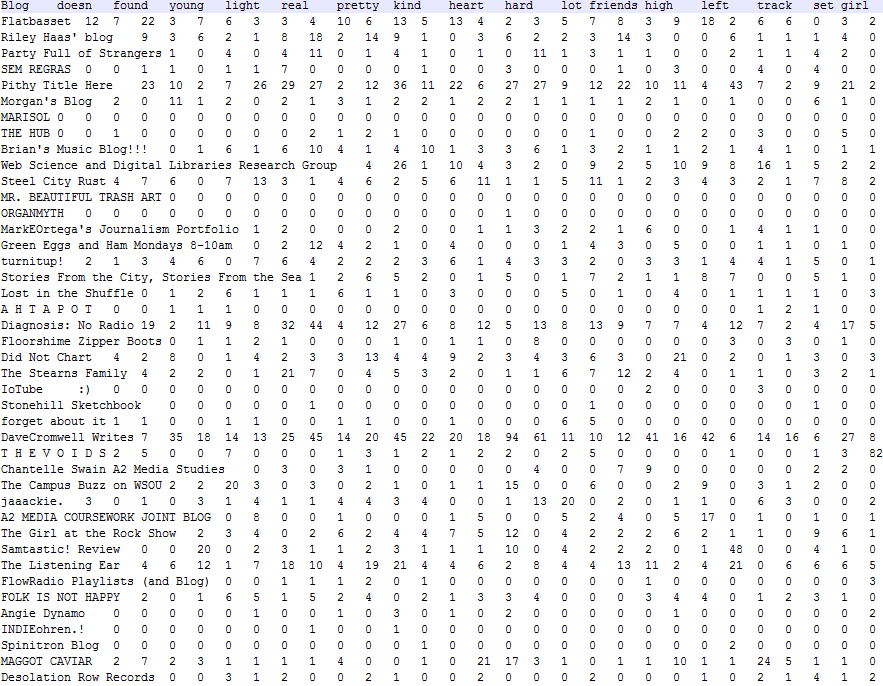
\includegraphics[scale=0.8]{input1.png}
        \caption{Sample Blogdata}
        \label{Sample1}
    \end{center}
\end{figure}
\newpage
\subsection{Outputs}

\subsubsection{Neighbors of F-Measure}
\begin{figure}[ht]    
    \begin{center}
        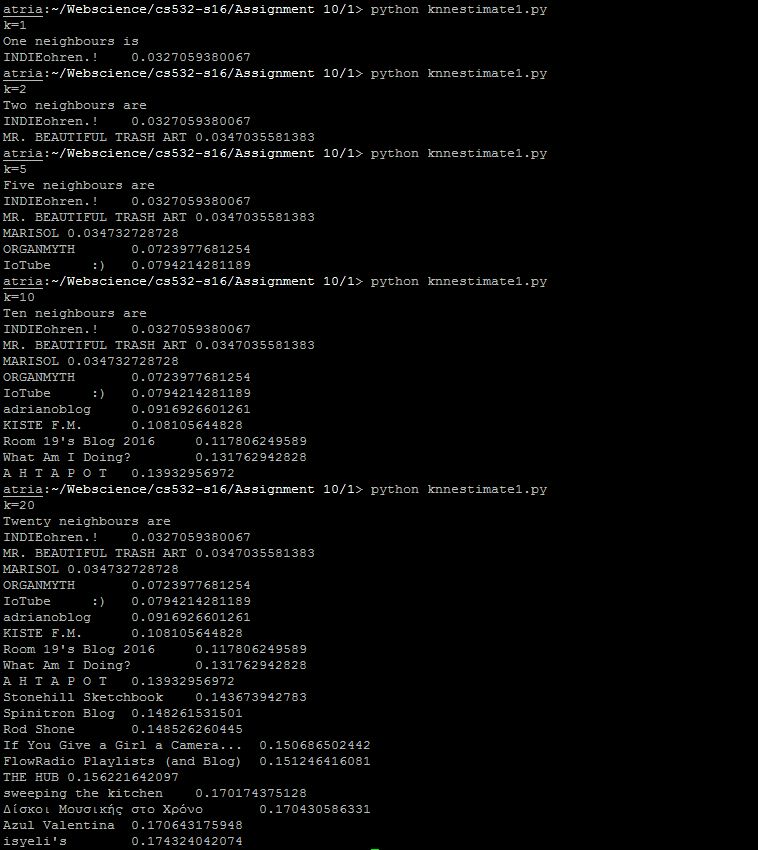
\includegraphics[scale=0.7]{fmeasureneighbours.png}
        \caption{Neighbors of F-Measure}
        \label{Sample2}
    \end{center}
\end{figure}
\newpage

\subsubsection{Neighbors of Ws-dl}
\begin{figure}[ht]    
    \begin{center}
        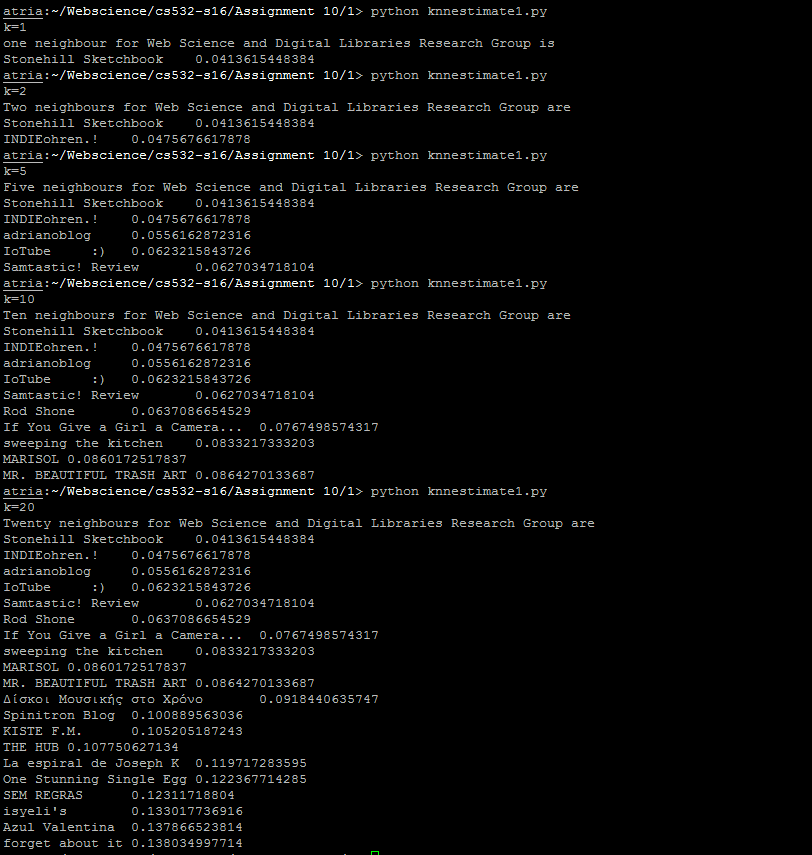
\includegraphics[scale=0.7]{wsdlneighbours.png}
        \caption{Neighbors of Ws-dl}
        \label{Sample3}
    \end{center}
\end{figure}
\newpage

